\documentclass[conference,a4paper]{IEEEtran}

% % --- Patch de redéfinition propre pour 15pt ---
% \makeatletter
% % On redéfinit \normalsize avec un corps de 15pt et un interligne (leading) de 18pt
% \renewcommand{\normalsize}{\@setfontsize\normalsize{15pt}{18pt}}
% % On applique immédiatement le changement pour le reste du préambule
% \normalsize 
% \makeatother
% % -----------------------------------------------

\usepackage[utf8]{inputenc}
\usepackage{cite}
\usepackage{amsmath,amssymb,amsfonts}
\usepackage{subcaption}
\usepackage{graphicx}
\usepackage{textcomp}
\usepackage{xcolor}
\usepackage{booktabs}
\usepackage{hyperref}
\hypersetup{hidelinks}
\usepackage{multirow}
\usepackage{mathtools}
\usepackage{flushend}
\usepackage{pgfplots}
\pgfplotsset{compat=newest}
\usetikzlibrary{arrows.meta,calc,positioning}

\definecolor{myred}{HTML}{D62728}
\definecolor{mygreen}{HTML}{2CA02C}
\definecolor{methodpurple}{HTML}{6F4C9B}
\definecolor{methodblue}{HTML}{2F6DAE}
\definecolor{methodorange}{HTML}{D97904}
\definecolor{methodgreen}{HTML}{2B8A6E}

%\hyphenation{op-tical net-works semi-conduc-tor}

\newcommand{\eg}{\textit{e.g., }}
\newcommand{\ie}{\textit{i.e., }}
\newcommand{\etal}{\textit{et al. }}
\newcommand{\norme}[1]{\left\lVert #1 \right\rVert}
\newcommand{\module}[1]{\left| #1 \right|}
\newcommand{\Frangi}{\textnormal{\textsc{Frangi}}}
\newcommand{\Hess}{\mathcal{H}}
\newcommand{\nom}[1]{\textsc{#1}}
\newcommand{\matnorm}[1]{\left\lvert\mkern-2mu\left\lvert\mkern-2mu\left\lvert #1 \right\rvert\mkern-2mu\right\rvert\mkern-2mu\right\rvert}
\newcommand{\ceremamark}{\raisebox{0pt}[0pt][0pt]{\textsuperscript{\footnotesize\textdegree}}}

\ifdefined\CameraReadyVersion
\makeatletter
\def\ps@IEEEtitlepagestyle{%
  \def\@oddfoot{\mycopyrightnotice}%
  \def\@evenfoot{}%
}
\def\mycopyrightnotice{%
  {\footnotesize 979-8-3195-3697-6/26/\$31.00~\copyright~2026 IEEE\hfill}
  \gdef\mycopyrightnotice{}%
}
\makeatother
\fi

\begin{document}

\ifdefined\CameraReadyVersion
\pagestyle{empty}
\else
\pagenumbering{arabic}
\pagestyle{plain}
\fi

\title{Multi-Modal, Training-Free Crack Extraction {via} Generalized Frangi Graph}

\author{
\IEEEauthorblockN{Louis \textsc{Hauseux}\IEEEauthorrefmark{1},
Raphaël \textsc{Antoine}\ceremamark,
Philippe \textsc{Foucher}\ceremamark,
Pierre \textsc{Charbonnier}\ceremamark, and
Josiane \textsc{Zerubia}\IEEEauthorrefmark{1}}
\IEEEauthorblockA{\IEEEauthorrefmark{1}\textit{Inria, Université Côte d'Azur, Ayana team, France}\\
\ceremamark\textit{Cerema, ENDSUM research team, France}\\
Corresponding author: Louis Hauseux (louis.hauseux@inria.fr)}
}

\maketitle
\ifdefined\CameraReadyVersion\else
\thispagestyle{plain}
\fi

\begin{abstract}
Automatic crack extraction is essential for both infrastructure inspection and geosciences, but annotated crack data remain scarce and domain shifts are frequent.
We address the problem of extracting a crack network from one or several scalar modalities, without training. 

To do so, we generalize the classical \Frangi{} vesselness filter from a pixel-wise operator to a pairwise spatial graph. While the standard filter is limited to independent pixel-wise geometry, our formulation enriches this description by explicitly encoding the orientation alignment between neighboring pixels, alongside elongation and contrast. The final crack network is then extracted through a graph pipeline combining minimum spanning tree reduction and similarity-weighted tree centrality.


While supervised models perform best on clean, in-distribution data, our geometry-driven framework degrades more slowly than a state-of-the-art deep-learning method under the tested synthetic perturbations.
\end{abstract}

\begin{IEEEkeywords}
Crack detection, multi-modal fusion, \Frangi{} filter, graph, minimum spanning tree, tree centrality
\end{IEEEkeywords}

\section{Introduction}

Reliable crack mapping is needed for civil infrastructure inspection and for monitoring geological hazards such as landslides, faults and subsidence \cite{bird2016coastal}. In practice, many crack maps are still produced or corrected manually, which is slow, subjective and difficult to scale. Automatic extraction is difficult because cracks are thin, discontinuous, and are often low-contrast structures whose appearance varies with the sensor, material, illumination, surface roughness and acquisition geometry.

Deep learning methods have become the dominant approach for crack segmentation. They perform well when training and test images follow the same distribution, but they require annotated data and may fail under sensor or domain shifts \cite{JosianeGANCrack2020,SOTACrack2020, Zhang2025Review}. 
This limitation is especially relevant for multi-modal crack analysis, where public benchmarks with clean, well-aligned visible, depth or thermal modalities remain rare.


This paper takes a complementary direction: % Rather than strictly competing with learned architectures on narrow training domains,
Our framework provides an interpretable, training-free extraction pipeline. It addresses multi-modal scenarios for which annotations are not available. In this setting, creating ground truth is very expensive.
Our method can directly assist domain experts (\eg geophysicists) and accelerate dataset annotation.

% The contribution is threefold. First, we formulate the crack extraction task as the recovery of a graph-like skeleton from scalar modalities under an explicit dark-ridge prior%\footnote{Dark-ridge prior which can become bright-ridge prior thanks to a simple modality inversion.}
% . Second, we generalize the \Frangi{} filter \cite{Frangi1998} from a pixel-wise vesselness response to a pairwise graph similarity using second-order shape, contrast and alignment terms. Third, we evaluate this graph formulation on FIND \cite{FIND2022} and on two geological image sets, including comparisons with supervised models on clean and noisy data.


Our main contributions are as follows: 
%(1) we formulate the crack extraction task as the recovery of a graph-like skeleton from scalar modalities under an explicit dark-ridge prior; 
(1) We generalize the \Frangi{} filter \cite{Frangi1998} from a pixel-wise vesselness response to a pairwise graph similarity using second-order shape, contrast and alignment terms, together with normalized multi-modal Hessian fusion;
(2) We evaluate our complete algorithm on the FIND benchmark \cite{FIND2022} and on two geological image sets, including comparisons with supervised models on clean and noisy data.
The contribution lies in coupling these established components through the pairwise \Frangi{} graph.

\section{Related Work}

\subsection{Classical Curvilinear Filters}
Multi-scale Hessian filters are a standard tool for enhancing curvilinear structures. The classical \Frangi{} vesselness filter \cite{Frangi1998} uses the eigensystem of a smoothed Hessian matrix to assess whether a pixel belongs to a tubular structure, following related work such as \textsc{Sato}'s line filter \cite{Sato1998}. These methods are fast and interpretable, but they are local: They evaluate pixels independently and can fragment under noise or textured backgrounds. Our method keeps the Hessian geometry but moves the decision from isolated pixels to edges of a spatial graph.
Our preliminary study \cite{BibiStrasbourg} considered two single-modal geological images. Here we add normalized multi-modal fusion, evaluate clean and noisy FIND data, and include a second geological setting.

\subsection{Deep Crack Segmentation}
Deep learning architectures such as U-Net \cite{Unet2015}, DeepCrack \cite{DeepCrack2019}, CrackFormer \cite{CrackFormer2021} and recent diffusion models such as CrackSegDiff \cite{CrackSegDiff2024} have achieved strong crack segmentation results. Their main practical weakness is their dependence on annotations. A recent survey by \textsc{Zhang} \emph{et al}. \cite{Zhang2025Review} also emphasizes poor cross-domain robustness when sensors, materials or acquisition conditions change. This motivates training-free alternatives and hybrid strategies that can operate when annotations are not available.

\subsection{Multi-Modal Fusion}
In machine learning, multi-modal fusion is usually implemented by channel concatenation, intermediate feature fusion or late prediction fusion. These choices depend on the network architecture and on the modalities available at training time. Here, fusion is performed at the operator level: Each modality contributes a normalized Hessian, and the fused Hessian is processed by the same graph pipeline regardless of the number of modalities.

\section{Methodology}

\subsection{Problem Formulation and Skeleton Output}
Let $\Omega\subset\mathbb Z^2$ be the image grid and let
\begin{equation}
    \mathcal I=\{I^{(m)}:\Omega\to\mathbb R\}_{m\in\mathcal M}
\end{equation}
be one or several scalar modalities, such as visible intensity, depth/range or thermal infrared images. The output is a set of pixels $\widehat\Gamma\subset\Omega$ representing the crack skeleton. We use ``skeleton'' in the standard image-analysis sense: A one-pixel-wide centerline representation that preserves the main connectivity and branches of a thin object; thick masks used for evaluation are skeletonized with the implementation reported in \cite{Lee1994, SciKitSkeletonization}.

The method assumes that the crack of interest is visible as a dark curvilinear ridge. If a sensor encodes cracks as bright ridges, the modality can be inverted before processing. 
Figure~\ref{fig:method_overview} summarizes the processing chain.
%If the sign or contrast is inconsistent, the image is outside the stated task rather than a counterexample to the graph extraction itself.

\begin{figure}[!t]
    \centering
    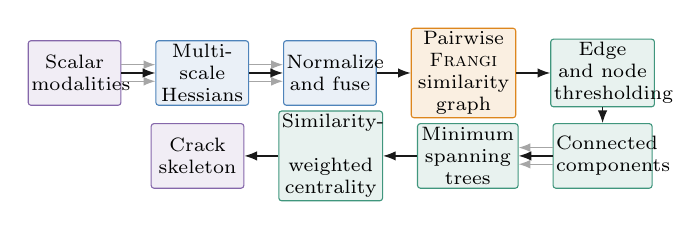
\begin{tikzpicture}[
        stage/.style={
            draw=black!65,
            rounded corners=1pt,
            align=center,
            text width=1.10cm,
            minimum height=0.82cm,
            inner sep=1.1pt,
            font=\scriptsize
        },
        problem/.style={stage, draw=methodpurple!85, fill=methodpurple!10},
        features/.style={stage, draw=methodblue!85, fill=methodblue!10},
        similarity/.style={stage, draw=methodorange!90, fill=methodorange!12},
        extraction/.style={stage, draw=methodgreen!90, fill=methodgreen!11},
        flow/.style={-{Latex[length=1.6mm]}, line width=0.45pt, draw=black!90},
        optional/.style={-{Latex[length=1.5mm]}, line width=0.38pt, draw=black!35},
        node distance=2mm and 4.3mm
    ]
        \node[problem] (inputs) {Scalar\\modalities};
        \node[features, right=of inputs] (hessians) {Multi-scale\\Hessians};
        \node[features, right=of hessians] (fusion) {Normalize\\and fuse};
        \node[similarity, text width=1.25cm, right=of fusion] (graph) {Pairwise \Frangi{}\\similarity graph};
        \node[extraction, text width=1.24cm, right=of graph] (pruning) {Edge and node\\thresholding};
        \node[extraction, text width=1.18cm, below=of pruning] (components) {Connected\\components};
        \node[extraction, text width=1.20cm, left=of components] (mst) {Minimum\\spanning trees};
        \node[extraction, text width=1.24cm, left=of mst] (centrality) {Similarity-\\weighted\\centrality};
        \node[problem, left=of centrality] (skeleton) {Crack\\skeleton};

        \draw[optional] ([yshift=3pt]inputs.east) -- ([yshift=3pt]hessians.west);
        \draw[flow] (inputs.east) -- (hessians.west);
        \draw[optional] ([yshift=-3pt]inputs.east) -- ([yshift=-3pt]hessians.west);
        \draw[optional] ([yshift=3pt]hessians.east) -- ([yshift=3pt]fusion.west);
        \draw[flow] (hessians.east) -- (fusion.west);
        \draw[optional] ([yshift=-3pt]hessians.east) -- ([yshift=-3pt]fusion.west);
        \draw[flow] (fusion) -- (graph);
        \draw[flow] (graph) -- (pruning);
        \draw[flow] (pruning) -- (components);
        \draw[optional] ([yshift=3pt]components.west) -- ([yshift=3pt]mst.east);
        \draw[flow] (components.west) -- (mst.east);
        \draw[optional] ([yshift=-3pt]components.west) -- ([yshift=-3pt]mst.east);
        \draw[flow] (mst.west) -- (centrality.east);
        \draw[flow] (centrality.west) -- (skeleton.east);
    \end{tikzpicture}
    \caption{Overview of the proposed method. Colors correspond to Sections III-A--D (purple/blue/orange/green), and Section III-E summarizes the role of the processing steps. Parallel black and gray arrows indicate the modalities and retained components.}
    \label{fig:method_overview}
\end{figure}

\subsection{Multi-Scale Hessian Features}
For a modality $I^{(m)}$ and a Gaussian scale $\sigma$, the smoothed Hessian at $x\in\Omega$ is
\begin{equation}
\Hess_{\sigma}^{(m)}(x)=
\begin{pmatrix}
\partial_{xx}(G_\sigma*I^{(m)})(x) & \partial_{xy}(G_\sigma*I^{(m)})(x) \\
\partial_{xy}(G_\sigma*I^{(m)})(x) & \partial_{yy}(G_\sigma*I^{(m)})(x)
\end{pmatrix}.
\label{eq:hessian}
\end{equation}
Equivalently, the derivatives are computed by convolution with derivatives of the Gaussian kernel \cite{Lindeberg1998, Frangi1998}, 
\begin{equation}
\partial_{ab}(G_\sigma*I^{(m)})=(\partial_{ab}G_\sigma)*I^{(m)},\qquad a,b\in\{x,y\}.
\end{equation}
Since the Hessian matrix in \eqref{eq:hessian} is real and symmetric, we compute its eigenvalues $\lambda_1^\sigma(x),\lambda_2^\sigma(x)$, ordered as $|\lambda_1^\sigma(x)|\le |\lambda_2^\sigma(x)|$. The eigenvector associated with $\lambda_1^\sigma(x)$ gives the local longitudinal direction of the ridge.
For an elongated ridge, transverse curvature dominates longitudinal curvature, so $R_B^\sigma(x)=|\lambda_1^\sigma(x)|/|\lambda_2^\sigma(x)|$ is near zero; for a blob-like structure, the two magnitudes are comparable and $R_B^\sigma(x)$ approaches one. Classical \Frangi{} vesselness combines this geometry with curvature magnitude and sign at each pixel. Our graph retains these local cues while requiring compatible evidence and longitudinal directions at neighboring pixels.

For multi-modal inputs, each Hessian is normalized by the largest spectral norm \cite{Horn2012Matrix} in the image,
\begin{equation}
    \widehat{\Hess}_{\sigma}^{(m)}(x)
    =
    \frac{\Hess_{\sigma}^{(m)}(x)}{
    \max_{y\in\Omega}\matnorm{\Hess_{\sigma}^{(m)}(y)}_2},
\end{equation}
and the fused Hessian is
\begin{equation}
    \Hess_{\sigma}^{\mathrm{fused}}(x)=
    \sum_{m\in\mathcal M}w_m\widehat{\Hess}_{\sigma}^{(m)}(x),
    \qquad w_m\ge0,\quad \sum_m w_m=1.
\label{eq:fusion}
\end{equation}
All eigenvalues and orientations used below are computed from \eqref{eq:fusion}. 


We assume that the crack geometry is shared across modalities, whereas sensor-specific artifacts are largely uncorrelated. Under this assumption, averaging the normalized Hessians reinforces consistent structures and reduces modality-specific noise.


\subsection{Generalized \Frangi{} Similarity Graph}
We build a sparse spatial graph $G=(V,E)$ on candidate pixels $ V \subseteq \Omega$. We denote the distance between two candidate pixels by
\begin{equation}
    \rho_{ij}=\norme{x_i-x_j}_2.
\label{eq:spatial_distance}
\end{equation}
Pixels $x_i,x_j\in V$ are connected when
\begin{equation}
    0<\rho_{ij}\le R.
\end{equation}
The radius $R$ allows short interruptions caused by noise or local loss of contrast to be bridged, while $\rho_{ij}$ discourages long accidental jumps.

For a scale $\sigma\in\Sigma$, an edge $(i,j)$ is assigned a base similarity $S_{ij}^\sigma\in[0,1]$ as a product of three soft constraints.

\emph{Curvature evidence.} For dark ridges, the useful transverse curvature is $C_\sigma(x)=\max\{\lambda_2^\sigma(x),0\}$. The intensity term is
\begin{equation}
S_{\mathrm{int}}^\sigma(i,j)=
1-\exp\left[-\frac12\left(\frac{\sqrt{C_\sigma(x_i)C_\sigma(x_j)}}{s_{\mathrm{i}}}\right)^2\right].
\end{equation}
It requires strong positive transverse curvature at both endpoints; the geometric mean makes the edge weak when either endpoint lacks this evidence. This term carries the dominant information of the classical \Frangi{} response.

\emph{Shape refinement.} On the structures detected by $S_{\mathrm{int}}^\sigma$, both endpoints should also have a small \Frangi{} ratio. Blob-like responses are therefore down-weighted by
\begin{equation}
S_{\mathrm{shape}}^\sigma(i,j)=
\exp\left[-\frac12\left(\frac{R_B^\sigma(x_i)+R_B^\sigma(x_j)}{s_{\mathrm{s}}}\right)^2\right].
\end{equation}

\emph{Alignment refinement.} If $\theta^\sigma(x)$ is the angle of the longitudinal eigenvector, locally incompatible directions on that same curvature support are down-weighted by
\begin{equation}
S_{\mathrm{align}}^\sigma(i,j)=
\exp\left[-\frac12\left(\frac{\sin(\theta^\sigma(x_i)-\theta^\sigma(x_j))}{s_{\mathrm{a}}}\right)^2\right].
\end{equation}
The sine accounts for the fact that crack directions are unoriented: $\theta$ and $\theta+\pi$ describe the same local axis.

Thus $S_{\mathrm{shape}}^\sigma$ and $S_{\mathrm{align}}^\sigma$ refine, rather than replace, the curvature structures identified by $S_{\mathrm{int}}^\sigma$. We first take the strongest base similarity across scales,
\begin{equation}
S_{ij}^{(0)}=\max_{\sigma\in\Sigma}
S_{\mathrm{int}}^\sigma(i,j)
S_{\mathrm{shape}}^\sigma(i,j)
S_{\mathrm{align}}^\sigma(i,j),
\end{equation}
which compares the local appearance and geometry without yet penalizing separation. We then define the graph dissimilarity as the $[0,1]$-clipped value of $\rho_{ij}(1-S_{ij}^{(0)})$, and its complementary similarity:
\begin{equation}
\begin{aligned}
    d_{ij}
    &=\operatorname{clip}_{[0,1]}\!\left(\rho_{ij}(1-S_{ij}^{(0)})\right)\\
    &=\min\!\left\{1,\rho_{ij}(1-S_{ij}^{(0)})\right\},
    \qquad S_{ij}=1-d_{ij}.
\end{aligned}
\label{eq:distance}
\end{equation}
For unit-distance neighbors ($\rho_{ij}=1$), dissimilarity is simply the complement of the base similarity. Across a short gap, $\rho_{ij}>1$ raises the cost, discouraging an accidental long connection while still allowing a strongly supported interruption to be bridged; clipping keeps the result bounded. In the subsequent pipeline, $S_{ij}$ is used for graph thresholding and centrality, whereas $d_{ij}$ supplies the costs for the subsequent minimum spanning trees.

The parameter settings are empirically adapted to the datasets considered, described in Section~\ref{sec:datasets}. For FIND and the Palais des Papes, we use $s_{\mathrm{s}}=2$, $s_{\mathrm{i}}=1/4$, $s_{\mathrm{a}}=1/8$, $\Sigma=\{1,3,5,7\}$ and $R=3$. For the Vaches Noires images, the single-modal implementation uses $s_{\mathrm{s}}=1/2$, $s_{\mathrm{i}}=1/4$, $s_{\mathrm{a}}=1/8$, $\Sigma=\{1,3,5,7,9\}$ to cover wider visible fractures, with the same radius $R=3$ as in the preliminary study.

\subsection{Graph Extraction}
The extraction pipeline consists of four steps. First, edge thresholding keeps the strongest fraction $\tau_E$ of edges, ranked by $S_{ij}$. On this retained edge set, each node is scored by its maximum incident similarity; node thresholding then keeps the strongest fraction $\tau_V$ of nodes. To reduce tuning, all experiments tie the two retention factors, $\tau_E=\tau_V=\tau$.

Second, connected components are obtained from the remaining graph. FIND provides the prior that only one crack structure is of interest, so we retain the component with the largest number of pixels. Without this prior, we retain every component whose pixel count exceeds a prescribed fraction $\eta|\Omega|$ of the image pixels; $\eta$ is chosen from the minimum size of the structures one wishes to extract. The next two steps are applied separately to every retained component.


Third, a minimum spanning tree $\mathcal T$ \cite{Prim1957} is computed for each retained component using the dissimilarity $d_{ij}$. Each tree preserves the ``cheapest'' coherent connections and turns the locally thick response into a structure suitable for centerline extraction.

Fourth, we compute a similarity-weighted tree centrality \cite{Freeman1977}, unlike general-graph betweenness \cite{Brandes2001}. It takes $O(|V|)$: Breadth-first traversal records parents level by level; its reverse order accumulates subtree masses. Each vertex receives the weight
\begin{equation}
    w_i=\max_{j:(i,j)\in E}S_{ij}.
\end{equation}
After rooting the tree, let $\mathcal T_i$ be the subtree below $x_i$, $m_i=\sum_{x_k\in\mathcal T_i}w_k$, and $M=\sum_k w_k$. We use
\begin{equation}
    C_{\mathcal T}(x_i)=m_i(M-m_i).
\label{eq:tree_centrality}
\end{equation}
The highest-scoring vertex becomes the tree root, and the subtree masses are recomputed from it. The non-root scores follow \eqref{eq:tree_centrality} and are normalized, while the selected root is assigned score one. A branch is stopped when a child falls below the relative or absolute cutoff. Pixels on the main axis therefore remain, while short peripheral branches are removed.

Figure~\ref{fig:GlobalAnalysis} shows the intermediate maps for a FIND example. The positive-curvature map is close to a classical pixel-wise \Frangi{} response; the graph similarity is cleaner because it also enforces pairwise orientation compatibility.

\subsection{Role of the Components}
\label{sec:role_components}
%The pixel-wise curvature term corresponds to the classical Hessian evidence; the graph construction adds pairwise compatibility; the tree and centrality steps convert a locally thick response into a centerline. 
The construction starts with $S_{\mathrm{int}}$, which imposes strong positive transverse curvature $\lambda_2$ at both endpoints and contains the dominant \Frangi{} evidence. The other pairwise terms act on these detected structures as refinements: They discourage shapes and connections that do not match the crack prior. Table~\ref{tab:components} summarizes this progression.

\begin{table}[!ht]
    \centering
    \caption{The \Frangi{} evidence and its graph refinements.}
    \label{tab:components}
    \begin{tabular}{p{0.27\linewidth}p{0.63\linewidth}}
        \toprule
        \textbf{Component} & \textbf{Role in the extraction chain} \\
        \midrule
        $S_{\mathrm{int}}$ & Detects strong positive transverse curvature at both endpoints; provides the dominant classical \Frangi{} evidence. \\
        $S_{\mathrm{shape}}$ & On that support, penalizes blob-like responses and favors elongated structures. \\
        $S_{\mathrm{align}}$ & On that support, penalizes incompatible directions and accidental bridges. \\
        $\rho_{ij}$ & In $d_{ij}$, discourages long links between otherwise similar pixels. \\
        Weighted centrality & Selects pixels lying on the main centerline of the retained graph. \\
        \bottomrule
    \end{tabular}
\end{table}

The sensitivity parameters were selected empirically, starting from our preliminary study \cite{BibiStrasbourg}. We retained $s_{\mathrm{i}}$ and $s_{\mathrm{a}}$ and increased $s_{\mathrm{s}}$ from $1/2$ to $2$ for FIND and the Palais des Papes, allowing more variation in the \Frangi{} ratio, which is less stable than the curvature and orientation terms.

The scale set, radius and tied retention factor are fixed per dataset. We set $\Sigma$ from the expected crack-width range and $R$ from the largest gap that should be bridged; $\tau=\tau_E=\tau_V$ controls the sparsity--recall trade-off. We use $\tau=0.25$ for FIND and the Palais des Papes, and $\tau=0.30$ for Vaches Noires, following the preliminary study \cite{BibiStrasbourg}.


\section{Experiments}

\subsection{Datasets and Protocol}
\label{sec:datasets}
The quantitative evaluation uses FIND \cite{FIND2022}, a public benchmark with aligned intensity ($I$) and range ($R$) images for road-crack detection (and a third modality, ``filtered'' $F$, which is a clean post-processing of the range modality). We compare against CrackSegDiff \cite{CrackSegDiff2024}, a supervised diffusion model for multi-modal crack segmentation. For both compared methods, the same evaluation protocol is used: Dense masks are skeletonized before comparison and overlap metrics are computed with a fixed spatial tolerance.

We also report experiments on two geological image sets provided by Cerema. The first contains two annotated $512\times512$ visible UAV patches from the Vaches Noires landslide at Villers-sur-Mer (France). We call these evaluation patches \texttt{Test1} and \texttt{Test2}; they are separate from the $3760\times2058$ image used to adapt the U-Net baseline. The second set is a photogrammetric intensity-range pair acquired on the retaining wall of the Palais des Papes in Avignon (France).

\subsection{Metrics}
\label{sec:metrics}
For a ground truth set $A$ and a predicted set $B$, we use the \textsc{Jaccard} index \cite{Jaccard1901}, also known as Intersection over Union \cite{IoUDeepLearning},
\begin{equation}
J(A,B)=\frac{\module{A\cap B}}{\module{A\cup B}},
\end{equation}
and the \textsc{Tversky} index \cite{Tversky1977},
\begin{equation}
T(A,B)=\frac{\module{A\cap B}}{\module{A\cap B}+\alpha\module{A\setminus B}+\beta\module{B\setminus A}},
\end{equation}
with $\alpha=1$ and $\beta=0.5$, so missed cracks are penalized more than false alarms. Since skeletons are one-pixel-wide, we dilate both skeletons by $3$ pixels before computing these overlap scores. This tolerance is empirical and only compensates for small localization shifts at the $256\times256$ FIND resolution. We also report a discrete \textsc{Wasserstein} distance \cite{Wasserstein, POT2017}, which measures spatial displacement between predicted and reference skeleton pixels.

\begin{figure}[!ht]
    \centering
    \begin{subfigure}[b]{0.24\linewidth}
        \centering
        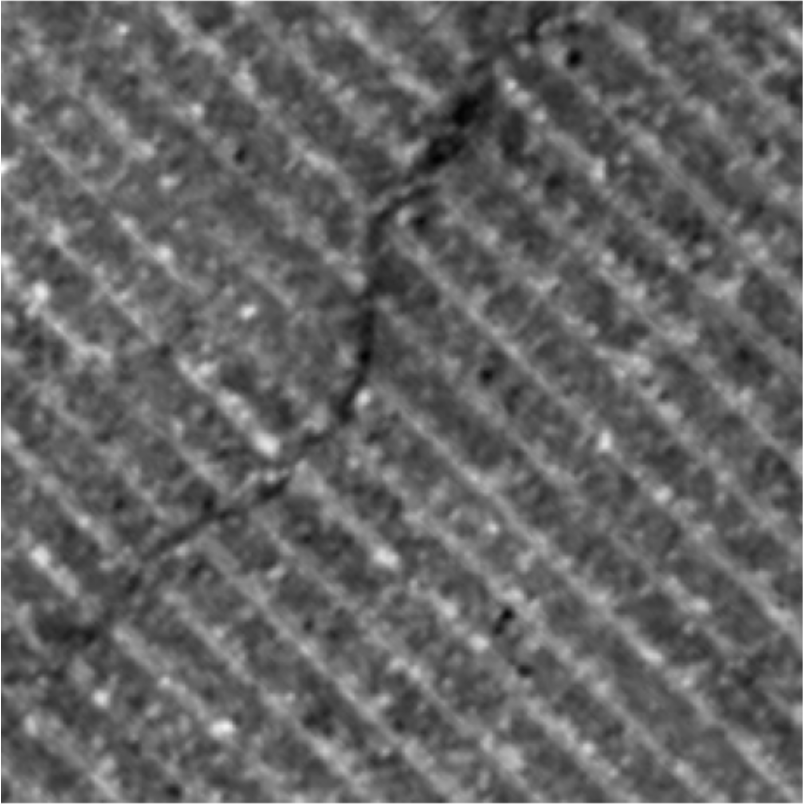
\includegraphics[width=\linewidth]{Intensity_1FIND.png}
        \caption{Intensity}
        \label{fig:intensity}
    \end{subfigure}
    \hfill
    \begin{subfigure}[b]{0.24\linewidth}
        \centering
        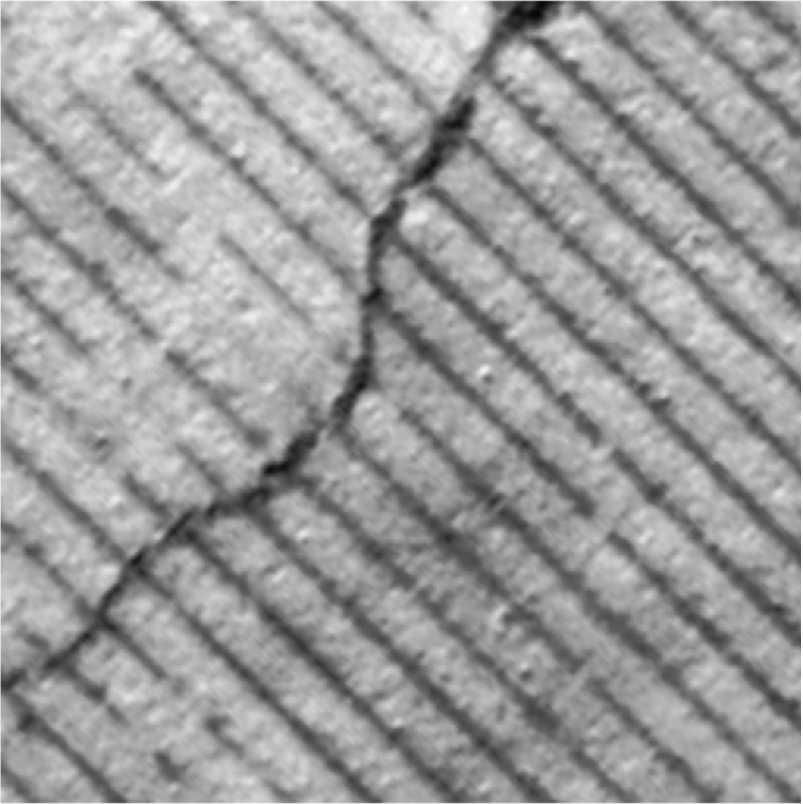
\includegraphics[width=\linewidth]{Range_1FIND.png}
        \caption{Range}
        \label{fig:range}
    \end{subfigure}
    \hfill
    \begin{subfigure}[b]{0.24\linewidth}
        \centering
        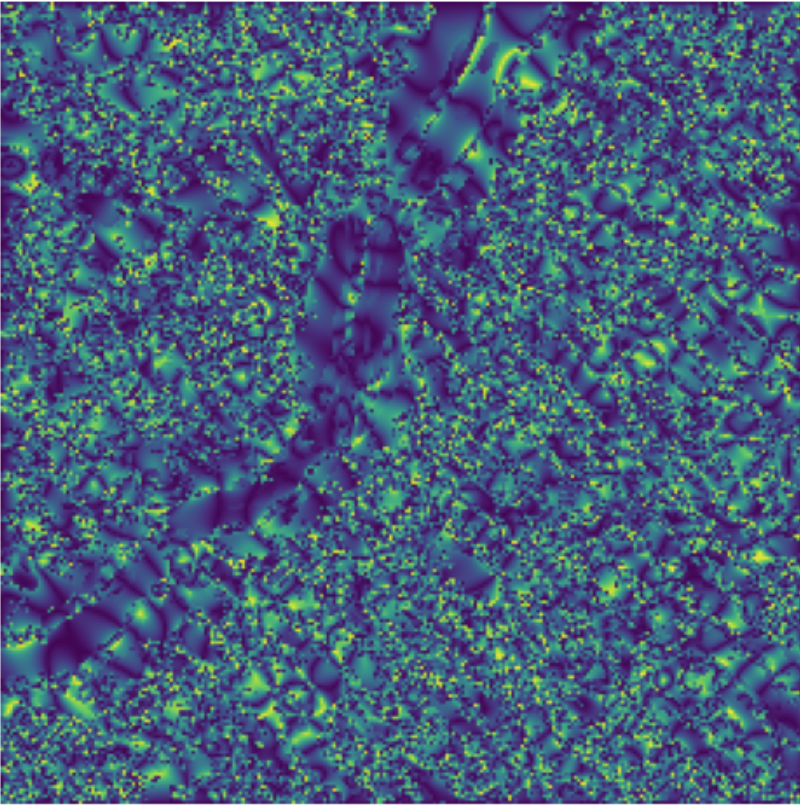
\includegraphics[width=\linewidth]{FrangiRatio_1FIND.png}
        \caption{$R_B$}
        \label{fig:frangiRatio}
    \end{subfigure}
    \hfill
    \begin{subfigure}[b]{0.24\linewidth}
        \centering
        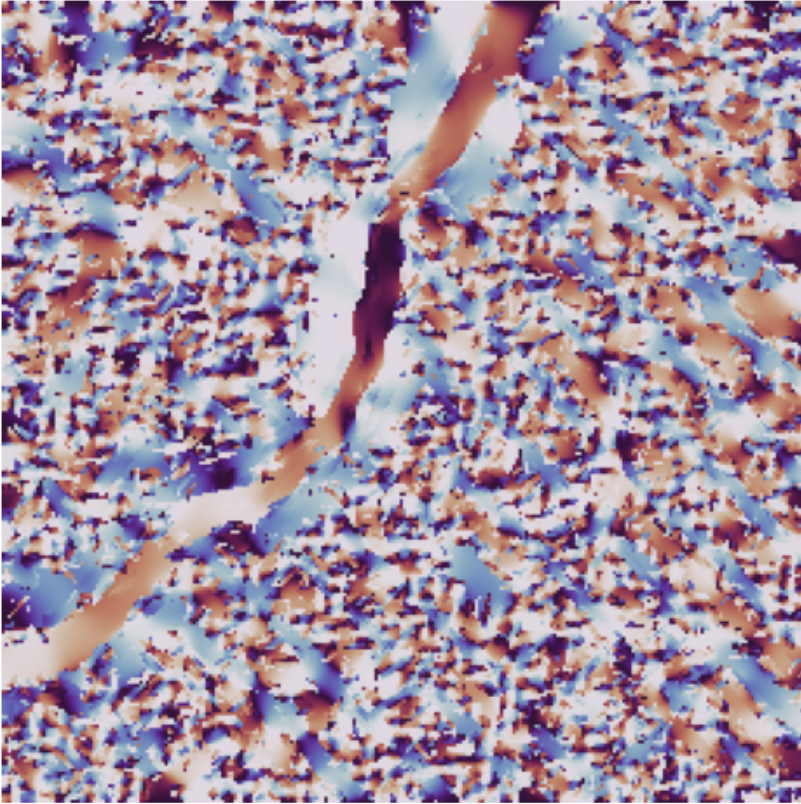
\includegraphics[width=\linewidth]{Angle_1FIND.png}
        \caption{Angle $\theta$}
        \label{fig:angle}
    \end{subfigure}

    \par\smallskip

    \begin{subfigure}[b]{0.24\linewidth}
        \centering
        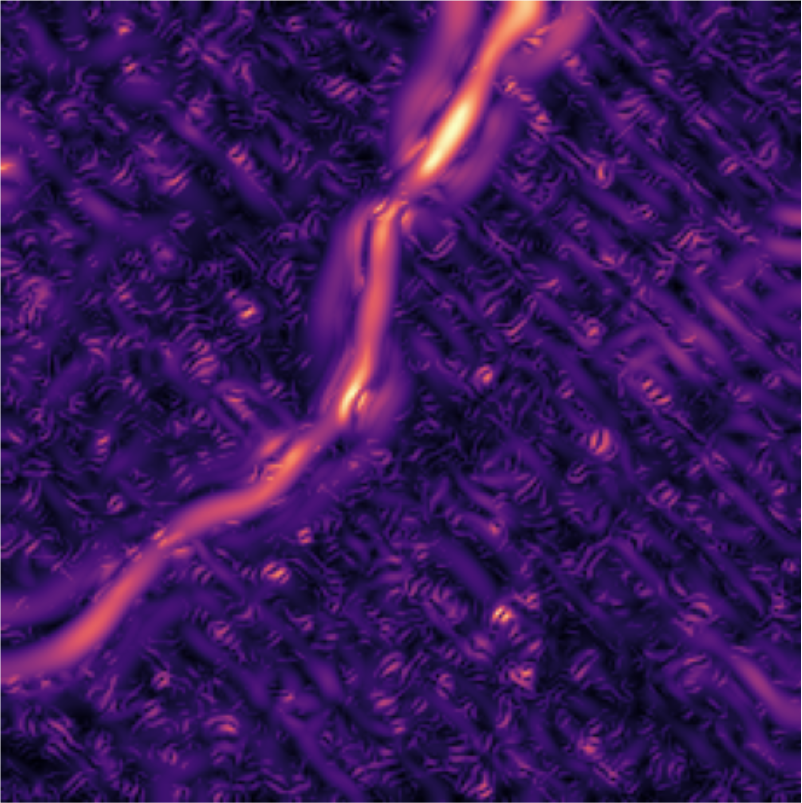
\includegraphics[width=\linewidth]{Int_1FIND.png}
        \caption{$\max(\lambda_2,0)$}
        \label{fig:frangi}
    \end{subfigure}
    \hfill
    \begin{subfigure}[b]{0.24\linewidth}
        \centering
        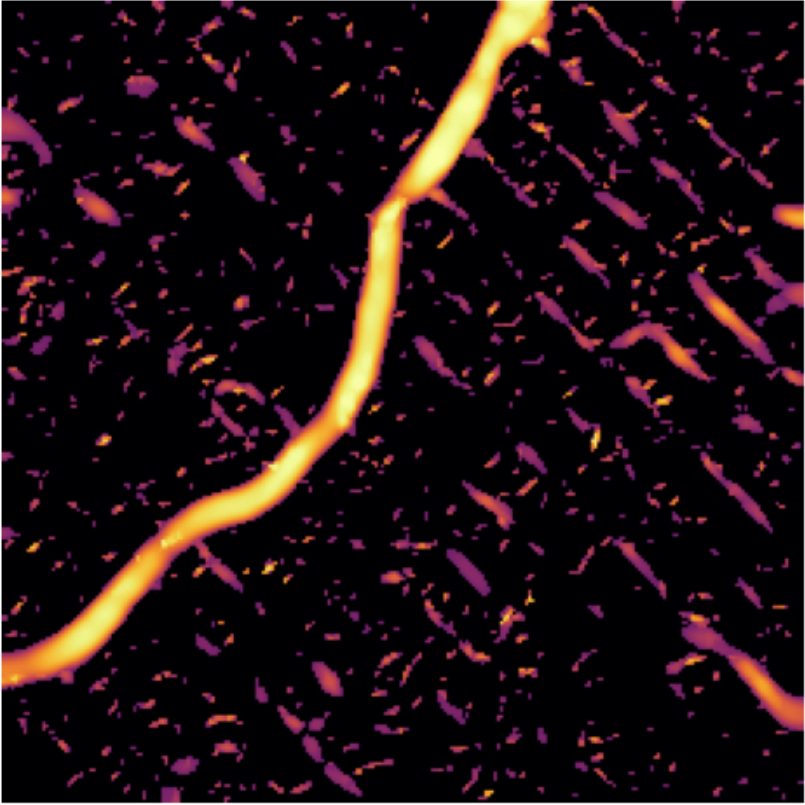
\includegraphics[width=\linewidth]{FrangiSim_1FIND.png}
        \caption{Similarity}
        \label{fig:similarity}
    \end{subfigure}
    \hfill
    \begin{subfigure}[b]{0.24\linewidth}
        \centering
        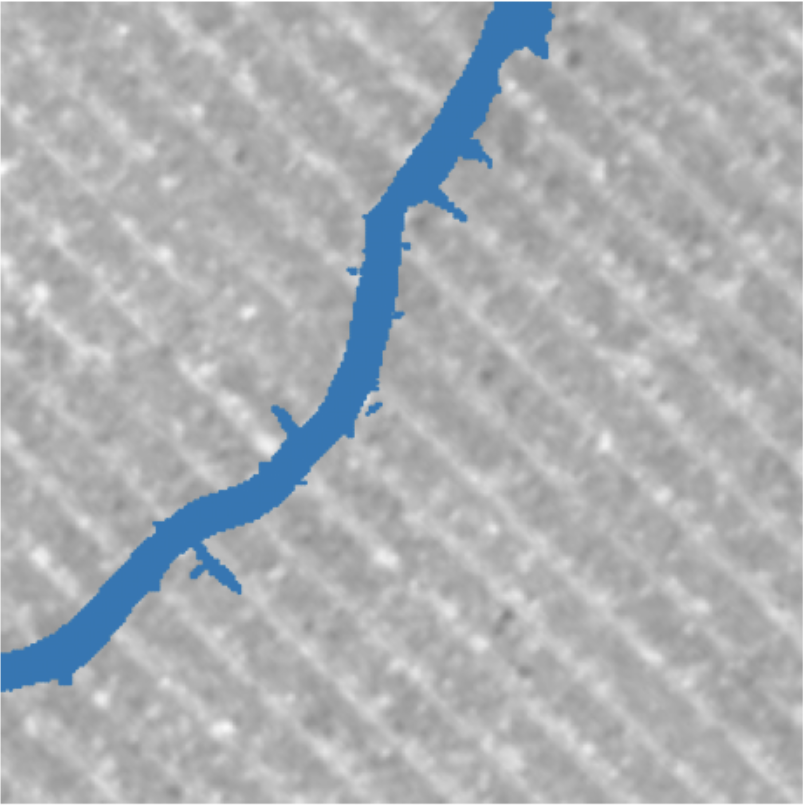
\includegraphics[width=\linewidth]{Cluster_1FIND.png}
        \caption{Larg. comp.}
        \label{fig:cluster}
    \end{subfigure}
    \hfill
    \begin{subfigure}[b]{0.24\linewidth}
        \centering
        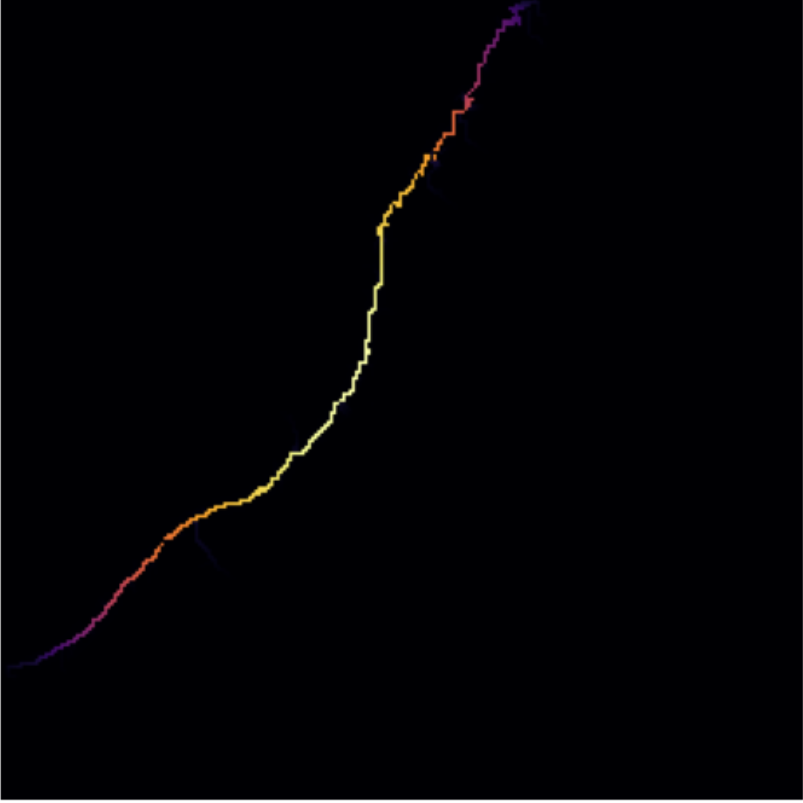
\includegraphics[width=\linewidth]{Betweenness_1FIND.png}
        \caption{Centrality}
        \label{fig:betweenness}
    \end{subfigure}

    \par\smallskip

    \begin{subfigure}[b]{0.24\linewidth}
        \centering
        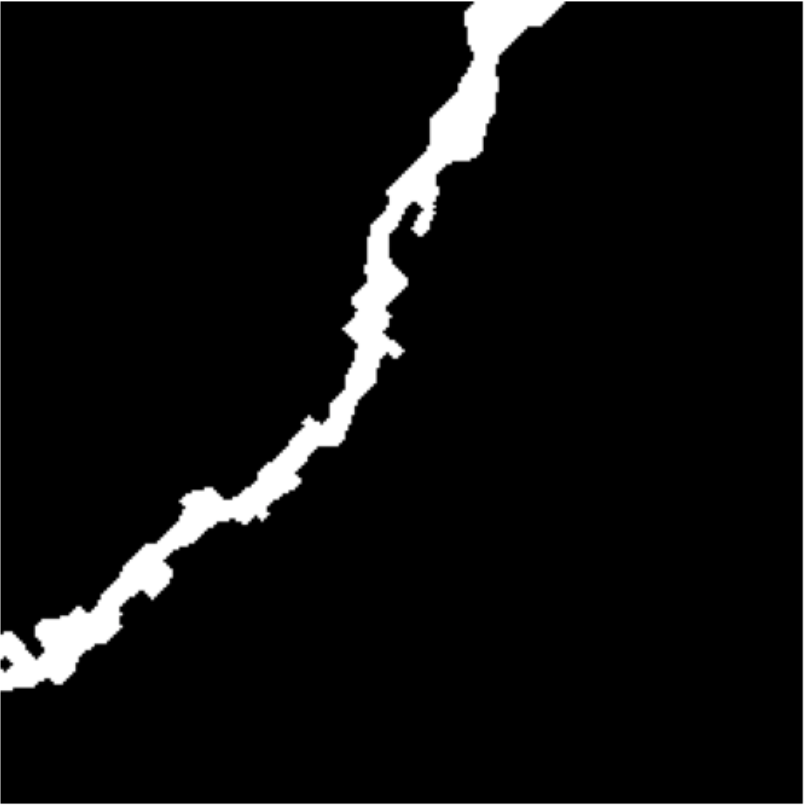
\includegraphics[width=\linewidth]{GroundTruth_1FIND.png}
        \caption{Ground truth}
        \label{fig:GT}
    \end{subfigure}
    \hfill
    \begin{subfigure}[b]{0.24\linewidth}
        \centering
        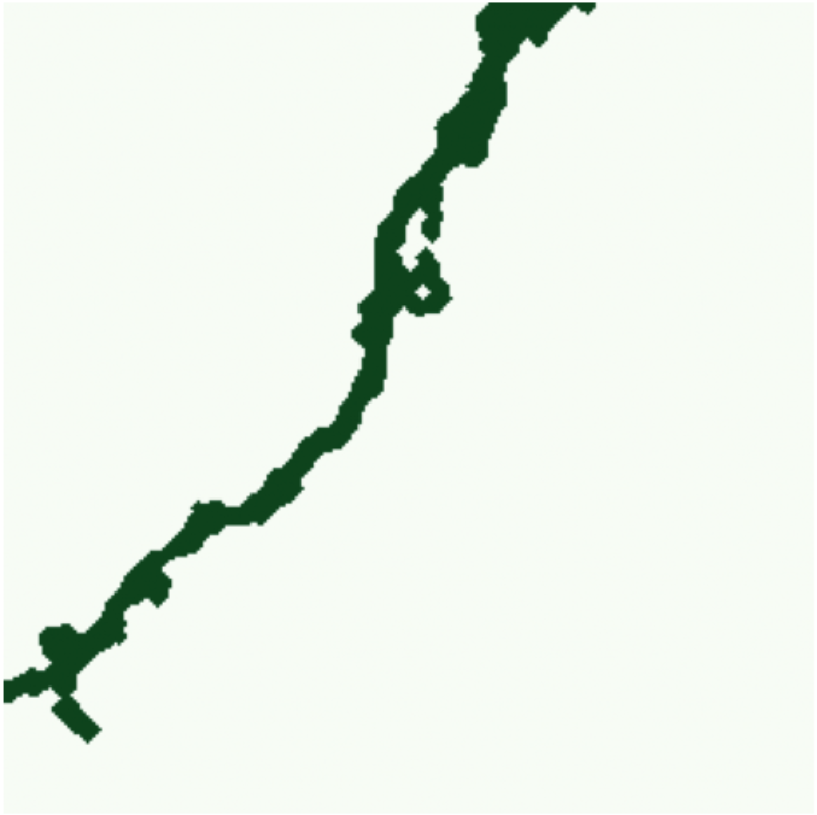
\includegraphics[width=\linewidth]{CrackSegDiff_1FIND.png}
        \caption{CrackSegDiff}
        \label{fig:CSD}
    \end{subfigure}
    \hfill
    \begin{subfigure}[b]{0.24\linewidth}
        \centering
        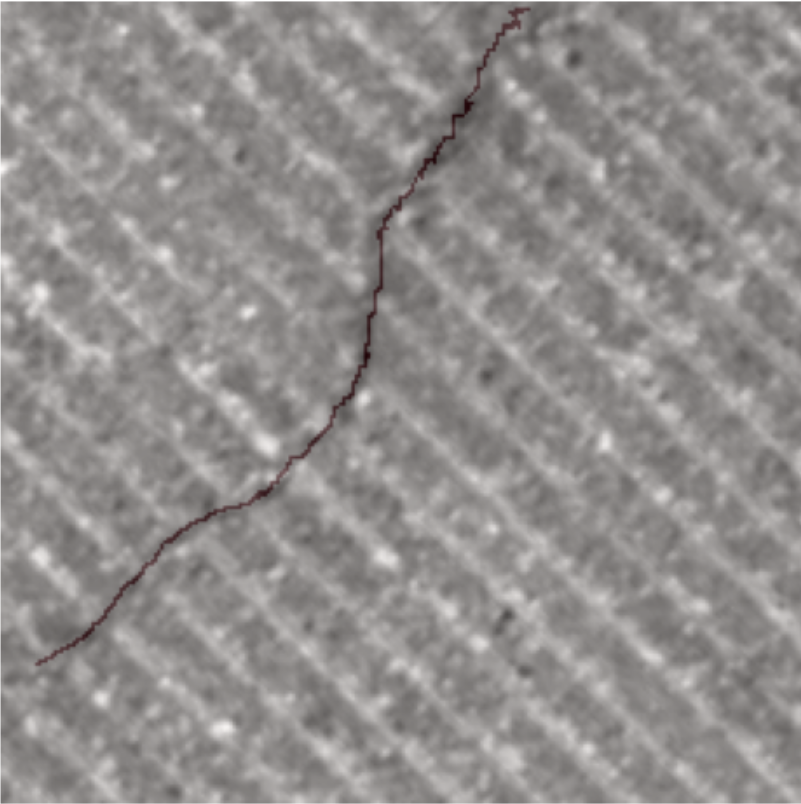
\includegraphics[width=\linewidth]{Resultat_1FIND.png}
        \caption{Our result}
        \label{fig:Resultat}
    \end{subfigure}
    \hfill
    \begin{subfigure}[b]{0.24\linewidth}
        \centering
        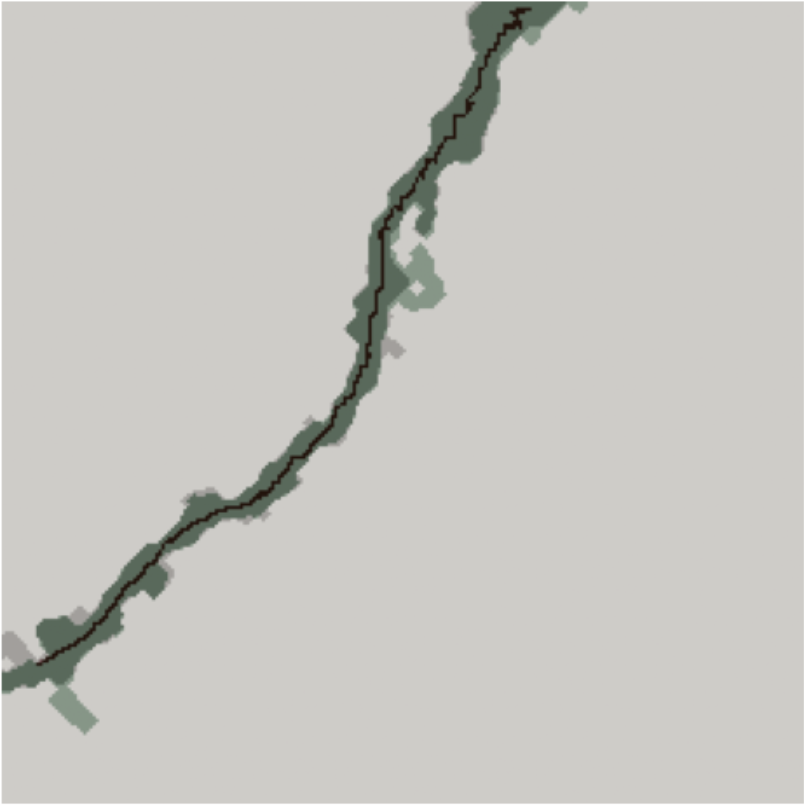
\includegraphics[width=\linewidth]{Overlay_1FIND.png}
        \caption{Overlay}
        \label{fig:Overlay}
    \end{subfigure}

    \caption{FIND example. \textbf{Top:} Intensity, Range, \Frangi{} ratio and orientation. \textbf{Middle:} Positive curvature, similarity, largest component and weighted centrality. \textbf{Bottom:} Ground truth, CrackSegDiff, ours (63\% \textsc{Jaccard}, 71\% \textsc{Tversky}, 8\,px \textsc{Wasserstein}) and overlay. At each $x\in V$, $|\lambda_2|$ selects the scale $\sigma$ at which $R_B$, $\theta$ and $\max(\lambda_2,0)$ are reported; pairwise similarity is the maximum over incident edges, each already maximized over $\sigma$.}
    \label{fig:GlobalAnalysis}
\end{figure}

\begin{figure*}[!t]
    \centering
    \begin{subfigure}[b]{0.315\textwidth}
        \centering
        \begin{tikzpicture}
            \node[anchor=south west, inner sep=0pt] (img) at (0,0) {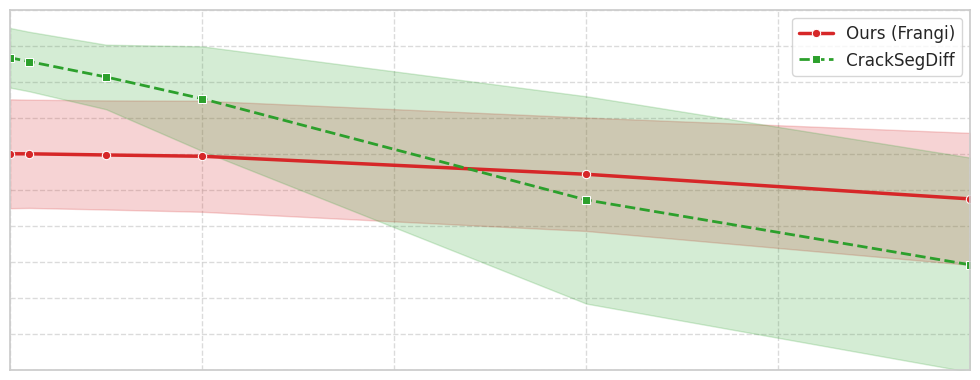
\includegraphics[width=0.84\linewidth]{Jaccard_noisy.png}};
            \useasboundingbox (img.south west) rectangle (img.north east);
            \draw[-latex, thin] (img.south west) -- (img.south east) -- ++(12pt,0) node[above left, inner sep=1pt, font=\scriptsize] {Noise};
            \draw[-latex, thin] (img.south west) -- (img.north west) -- ++(0,12pt) node[above, font=\scriptsize] {Score (\%)};
            \node[below left, font=\scriptsize] at (img.south west) {$0$};
            \node[below, font=\scriptsize] at (img.south east) {$0.5$};
            \node[left, font=\scriptsize] at (img.north west) {$100$};
        \end{tikzpicture}
        \caption{\textsc{Jaccard}}
    \end{subfigure}
    \hfill
    \begin{subfigure}[b]{0.315\textwidth}
        \centering
        \begin{tikzpicture}
            \node[anchor=south west, inner sep=0pt] (img) at (0,0) {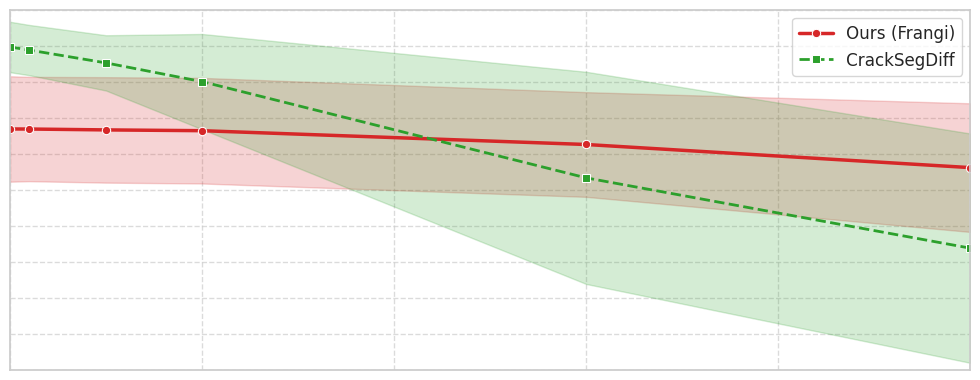
\includegraphics[width=0.84\linewidth]{Tversky_noisy.png}};
            \useasboundingbox (img.south west) rectangle (img.north east);
            \draw[-latex, thin] (img.south west) -- (img.south east) -- ++(12pt,0) node[above left, inner sep=1pt, font=\scriptsize] {Noise};
            \draw[-latex, thin] (img.south west) -- (img.north west) -- ++(0,12pt) node[above, font=\scriptsize] {Score (\%)};
            \node[below left, font=\scriptsize] at (img.south west) {$0$};
            \node[below, font=\scriptsize] at (img.south east) {$0.5$};
            \node[left, font=\scriptsize] at (img.north west) {$100$};
        \end{tikzpicture}
        \caption{\textsc{Tversky}}
    \end{subfigure}
    \hfill
    \begin{subfigure}[b]{0.315\textwidth}
        \centering
        \begin{tikzpicture}
            \node[anchor=south west, inner sep=0pt] (img) at (0,0) {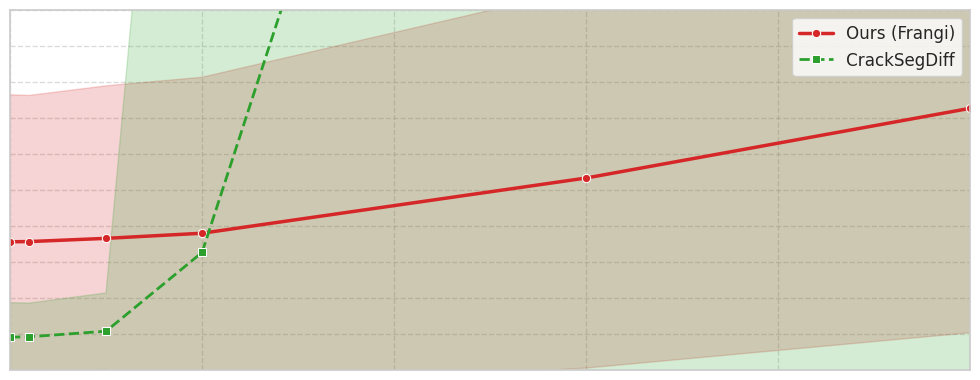
\includegraphics[width=0.84\linewidth]{Wasserstein_noisy.png}};
            \useasboundingbox (img.south west) rectangle (img.north east);
            \draw[-latex, thin] (img.south west) -- (img.south east) -- ++(12pt,0) node[above left, inner sep=1pt, font=\scriptsize] {Noise};
            \draw[-latex, thin] (img.south west) -- (img.north west) -- ++(0,12pt) node[above, font=\scriptsize] {Dist. (px)};
            \node[below left, font=\scriptsize] at (img.south west) {$0$};
            \node[below, font=\scriptsize] at (img.south east) {$0.5$};
            \node[left, font=\scriptsize] at (img.north west) {$100$};
        \end{tikzpicture}
        \caption{\textsc{Wasserstein}}
    \end{subfigure}
    \caption{Performance degradation on noisy FIND. Red: Proposed method; Green: CrackSegDiff. Shaded regions show standard deviation. The horizontal axis is the noise level $s$ (standard deviation of the Gaussians).}
    \label{fig:Results_noisy}
\end{figure*}


\subsection{FIND: Clean and Noisy Data}


Table~\ref{tab:ResultatsClean} compares the proposed method with CrackSegDiff on clean FIND images using intensity and range. 
As expected, CrackSegDiff achieves the highest overlap on the clean, in-distribution data it was trained on. However, our geometric formulation still recovers the main topology of the fracture networks without requiring any training data, demonstrating its viability as a training-free baseline.


\begin{table}[!ht]
    \centering
    \caption{Performance on clean FIND data}
    \label{tab:ResultatsClean}
    \begin{tabular}{@{}lccc@{}}
        \toprule
        Method & \textsc{Jaccard} & \textsc{Tversky} & \textsc{Wasserstein} \\
        \midrule
        Ours $(I+R)$ & 60\% & 68\% & 18 px \\
        CrackSegDiff & \textbf{87\%} & \textbf{90\%} & \textbf{5 px} \\
        \bottomrule
    \end{tabular}
\end{table}

The FIND dataset \cite{FIND2022} also contains a filtered range modality. Table~\ref{tab:ResultatsAblation} reports a modality contribution analysis for the proposed method. The filtered modality alone is strong, which shows the importance of clean, possibly pre-processed inputs for our method. Fusing intensity, range and filtered range gives the best result and supports the operator-level fusion strategy.


\begin{table}[!tb]
    \centering
    \caption{Modality contribution analysis for the proposed method on FIND. $I$: Intensity, $R$: Range, $F$: Filtered range.}
    \label{tab:ResultatsAblation}
    \begin{tabular}{@{}lccc@{}}
        \toprule
        Weights & \textsc{Jaccard} $\uparrow$ & \textsc{Tversky} $\uparrow$ & \textsc{Wasserstein} $\downarrow$ \\
        \midrule
        $I=1$ & 41\% & 48\% & 43 px \\
        $R=1$ & 54\% & 62\% & 20 px \\
        $F=1$ & 60\% & 68\% & 12 px \\
        $I=\tfrac12,R=\tfrac12$ & 60\% & 68\% & 18 px \\
        $I=\tfrac13,R=\tfrac13,F=\tfrac13$ & \textbf{63\%} & \textbf{71\%} & \textbf{11 px} \\
        \bottomrule
    \end{tabular}
\end{table}


To evaluate the framework's robustness to synthetic sensor noise, we artificially degrade the input modalities. Specifically, we perturb the intensity modality with multiplicative speckle noise to simulate surface reflectance variations, and corrupt the range modality with additive Gaussian noise to model instrumental measurement errors:

\begin{equation}
I_{\text{noisy}}(x) = I(x) \cdot (1+N(x)),
\end{equation}
\begin{equation}
R_{\text{noisy}}(x) = R(x) + N'(x),
\end{equation}

where $I(x)$ and $R(x)$ denote the original intensity and range signals at pixel $x$, respectively. 
$N(x),N'(x) \sim \mathcal N(0,s^2)$ are independent Gaussian random variables where $s^2$ measures the variance of the noise.
This protocol evaluates the robustness of our operator-level fusion to controlled sensor perturbations.

%To test robustness outside the clean training distribution, we add multiplicative speckle noise to intensity and additive Gaussian noise to range. 
Figure~\ref{fig:Results_noisy} reports the degradation curves, and Figure~\ref{fig:RobustesseNoisy} shows an example at a strong noise level. CrackSegDiff initially performs better, but its score decreases rapidly as noise increases. The proposed method starts lower but degrades more smoothly because the graph uses multi-scale curvature and orientation compatibility instead of learned appearance statistics alone.

\begin{figure}[!tb]
    \centering
    \begin{subfigure}[b]{0.24\linewidth}
        \centering
        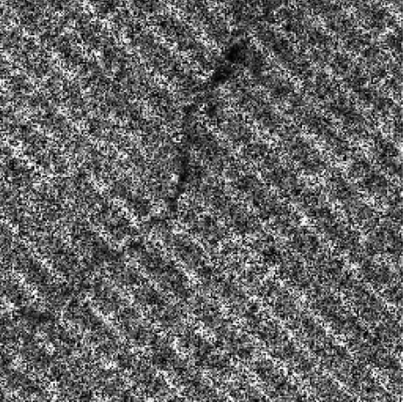
\includegraphics[width=\linewidth]{IntensityNoisy_1FIND.png}
        \caption{Noisy Int.}
        \label{fig:intensityNoisy}
    \end{subfigure}
    \hfill
    \begin{subfigure}[b]{0.24\linewidth}
        \centering
        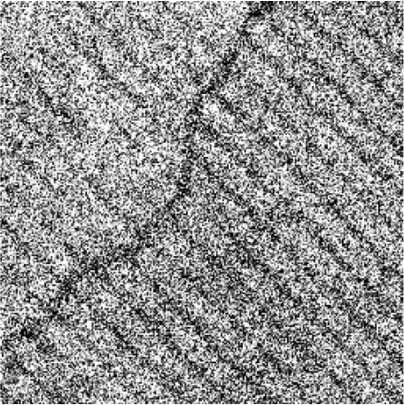
\includegraphics[width=\linewidth]{RangeNoisy_1FIND.png}
        \caption{Noisy Range}
        \label{fig:rangeNoisy}
    \end{subfigure}
    \hfill
    \begin{subfigure}[b]{0.24\linewidth}
        \centering
        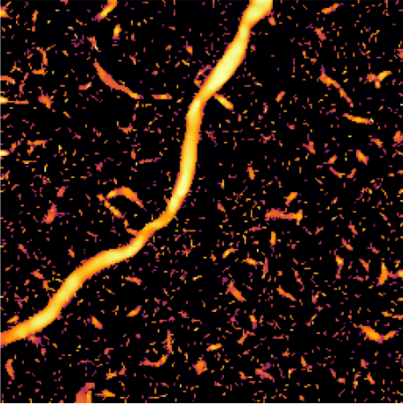
\includegraphics[width=\linewidth]{SimilarityNoisy_1FIND.png}
        \caption{Similarity}
        \label{fig:similarityNoisy}
    \end{subfigure}
    \hfill
    \begin{subfigure}[b]{0.24\linewidth}
        \centering
        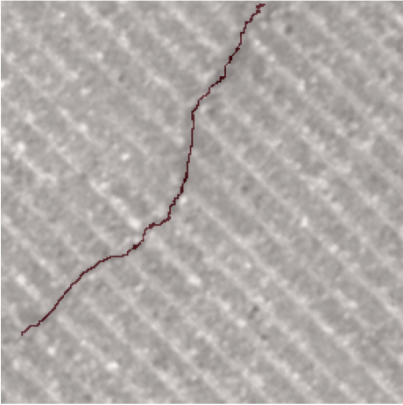
\includegraphics[width=\linewidth]{ResultatNoisy_1FIND.png}
        \caption{Our result}
        \label{fig:resultatNoisy}
    \end{subfigure}
    \caption{Noisy FIND example ($s=0.5$) with speckle noise on intensity and Gaussian noise on range. The graph similarity remains concentrated around the main crack.}
    \label{fig:RobustesseNoisy}
\end{figure}

\subsection{Geological Domain Shift}

The Vaches Noires data differ markedly from the road-crack FIND images and contain only a visible modality. We use $\Sigma=\{1,3,5,7,9\}$, $R=3$ and $\tau=0.3$ for both evaluation patches.
%The overall extraction pipeline is illustrated in Figure~\ref{fig:GlobalAnalysis}.

We compare against a U-Net baseline adapted by transfer learning \cite{UNetTransferLearningCracks2023} on an annotated $3760\times2058$ pixel image from the same area, following the common strategy used when only a small amount of domain-specific annotation is available. This ground truth annotation required approximately two days of work by an expert geophysicist. The proposed method uses only the visible image and no training annotation.

\begin{table}[!tb]
    \centering
    \caption{Quantitative comparison on the two annotated Vaches Noires patches.}
    \label{tab:vaches}
    \begin{tabular}{@{}llccc@{}}
        \toprule
        Image & Method & \textsc{Jaccard} $\uparrow$ & \textsc{Tversky} $\uparrow$ & \textsc{Wasserstein} $\downarrow$ \\
        \midrule
        \multirow{2}{*}{\texttt{Test1}}
        & Ours & 0.47 & 0.52 & \textbf{34 px} \\
        & U-Net + T.L. & \textbf{0.50} & \textbf{0.60} & 38 px \\
        \midrule
        \multirow{2}{*}{\texttt{Test2}}
        & Ours & 0.29 & 0.32 & 81 px \\
        & U-Net + T.L. & \textbf{0.34} & \textbf{0.36} & \textbf{60 px} \\
        \bottomrule
    \end{tabular}
\end{table}

\begin{figure}[!tb]
    \centering
    \begin{subfigure}[b]{0.485\linewidth}
        \centering
        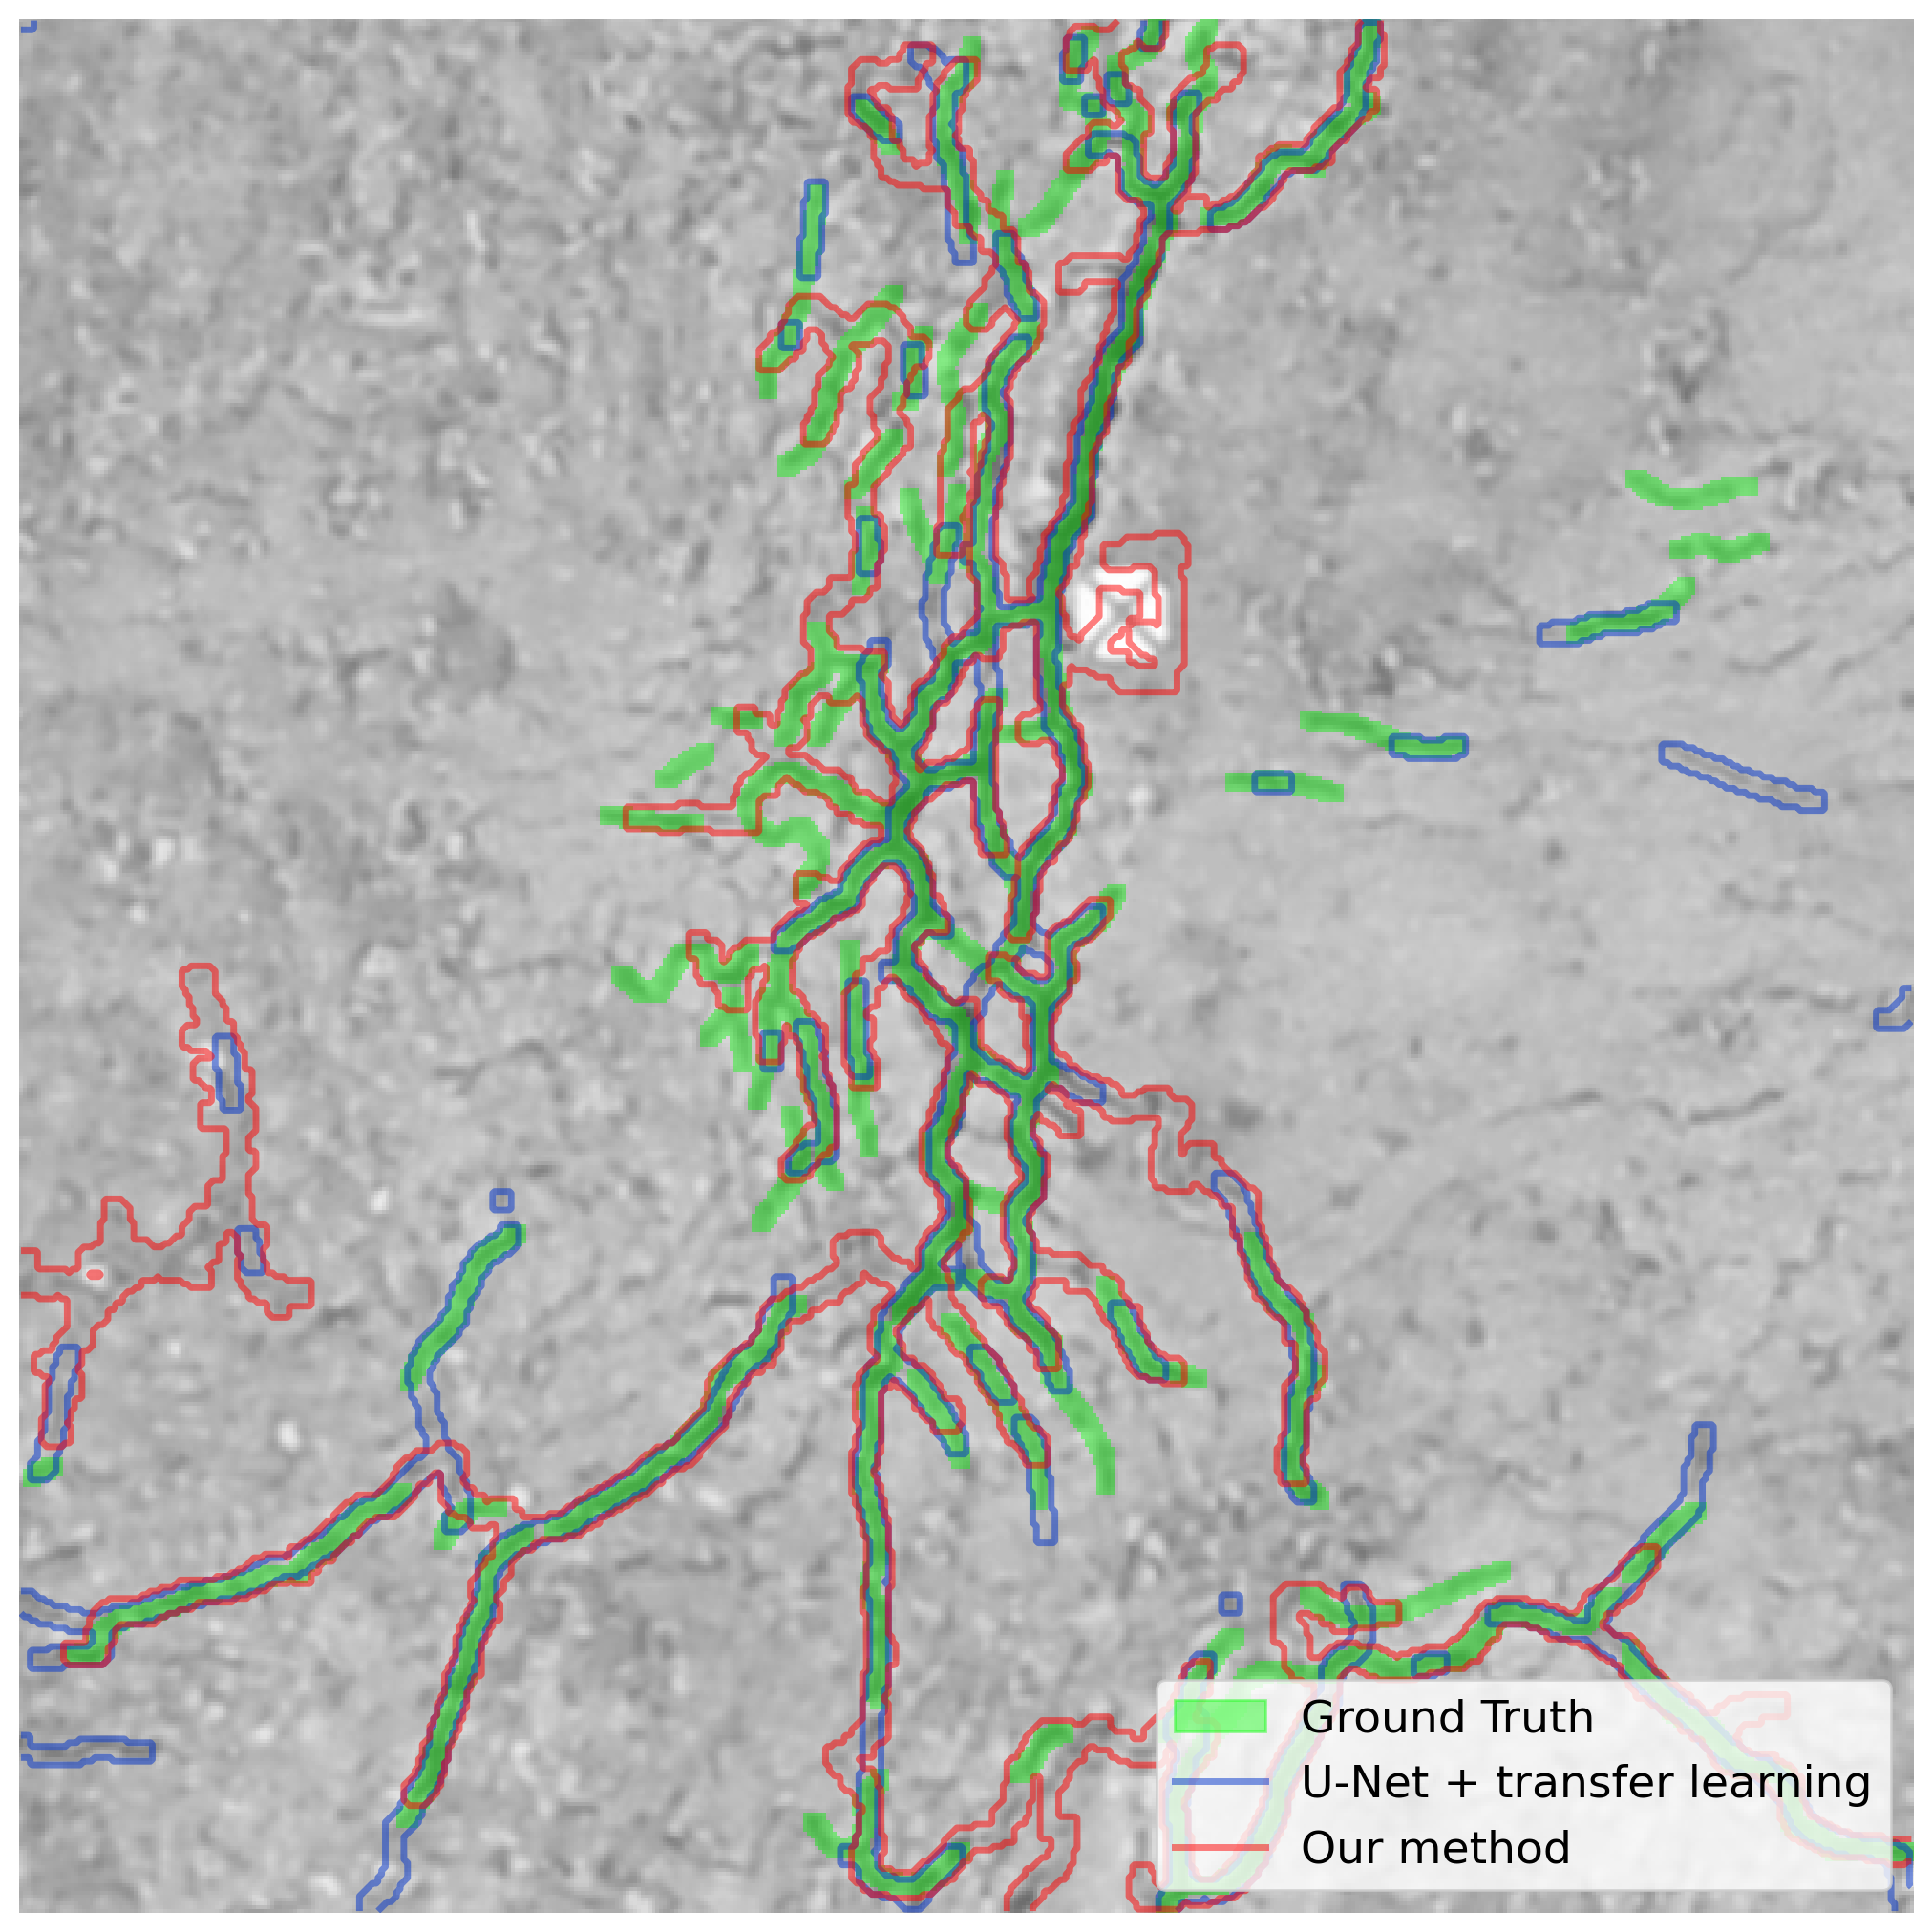
\includegraphics[width=\linewidth]{Test1_512_512_result.png}
        \caption{\texttt{Test1}}
        \label{fig:vaches_resultats1}
    \end{subfigure}
    \hfill
    \begin{subfigure}[b]{0.485\linewidth}
        \centering
        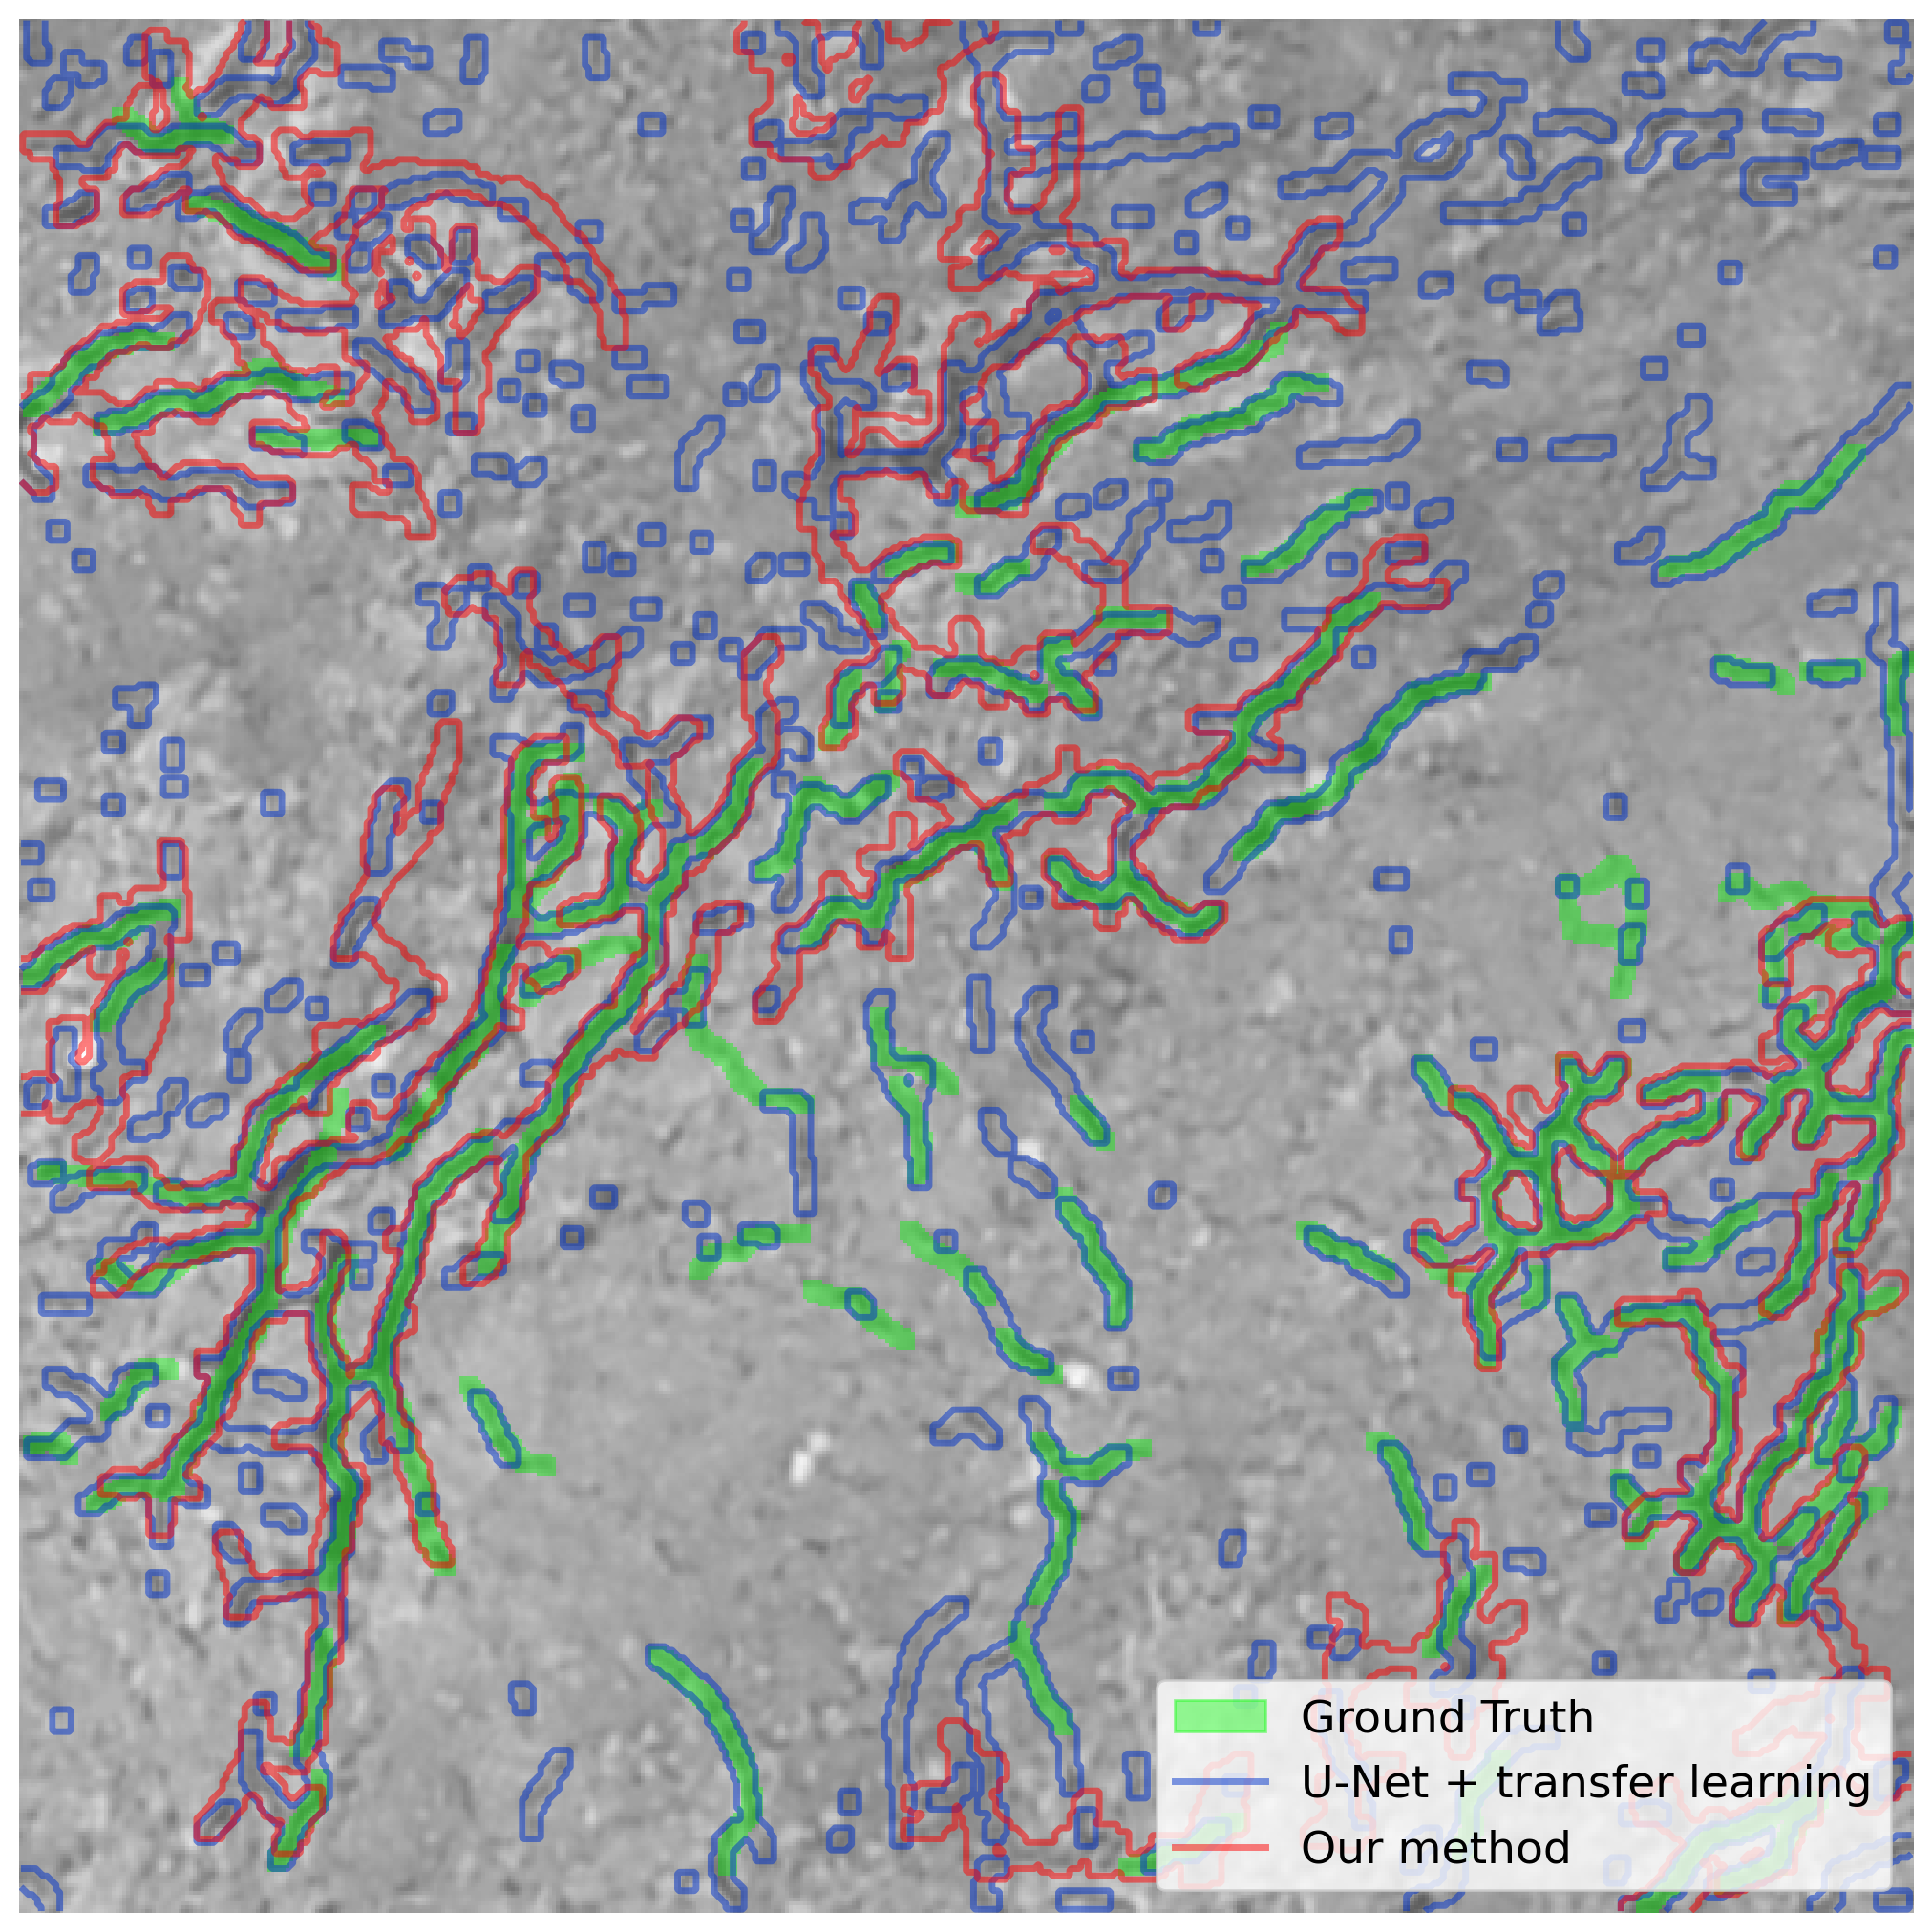
\includegraphics[width=\linewidth]{Test2_512_512_result.png}
        \caption{\texttt{Test2}}
        \label{fig:vaches_resultats2}
    \end{subfigure}
    \caption{Vaches Noires patches. Ground truth: Green; ours: Red; U-Net with transfer learning: Blue.}
    \label{fig:vaches_resultats}
\end{figure}

The supervised baseline gives slightly higher overlap scores on both patches, which is expected because it was adapted on a nearby annotated image. Our method uses no annotation and gives a lower \textsc{Wasserstein} distance on \texttt{Test1}. These two patches are useful transfer tests, but they are not enough to establish performance across domains.

We also apply the method to a fractured limestone wall at the Palais des Papes, using an orthoimage and a photogrammetric depth map. Figure~\ref{fig:PalaisDesPapes} shows that the main fracture is recovered without retraining; minor cracks are missed where depth resolution and contrast are insufficient.

\begin{figure}[!ht]
    \centering
    \begin{subfigure}[b]{0.32\linewidth}
        \centering
        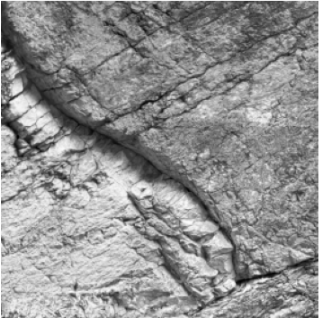
\includegraphics[width=\linewidth]{PalaisDesPapes.png}
        \caption{Intensity}
        \label{fig:intensityPapes}
    \end{subfigure}
    \hfill
    \begin{subfigure}[b]{0.32\linewidth}
        \centering
        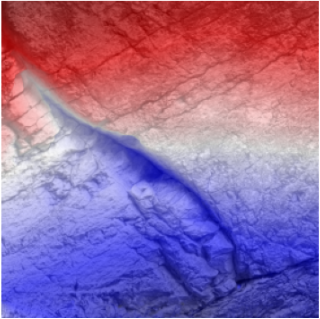
\includegraphics[width=\linewidth]{PalaisDesPapes_IntDepth.png}
        \caption{Int. + Range}
        \label{fig:rangePapes}
    \end{subfigure}
    \hfill
    \begin{subfigure}[b]{0.32\linewidth}
        \centering
        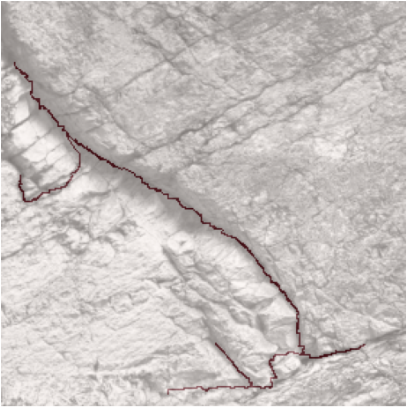
\includegraphics[width=\linewidth]{PalaisDesPapes_Result.png}
        \caption{Ours}
        \label{fig:resultatPapes}
    \end{subfigure}
    \caption{Palais des Papes wall: Intensity, depth overlay and extracted skeleton.}
    \label{fig:PalaisDesPapes}
\end{figure}

\section*{Code and Data Availability}
Code, notebooks and non-public data are available in the provided Frangi-EUVIP GitHub repository: \url{https://github.com/Ayana-Inria/Frangi-EUVIP}. FIND is public \cite{FIND2022}.

\section{Conclusion}
We presented a geometric, training-free method for multi-modal crack skeletonization. On clean FIND data, the supervised model performs better; under added noise, our graph method degrades more slowly. The geological results show that the method can be applied without retraining, but the evaluation is limited to two annotated patches and one qualitative case.

The editable graph supports semi-automatic annotation. Future priorities are direct comparisons with SAM \cite{Kirillov2023SAM} and CrackSAM \cite{Ge2024CrackSAM}, sensitivity tests on established datasets \cite{shi2016automatic}, and higher-order graph variants \cite{BibiAppliedNetworkScience}.

\section*{Acknowledgment}
The Inria authors were supported by Bpifrance (LiChIE, 2020--2025); the first author by Université Côte d'Azur through DS4H (ANR-17-EURE-0004) and 3IA (ANR-19-P3IA-0002).

\clearpage
\bibliographystyle{IEEEtran}
\bibliography{IEEEabrv,referencesThesis}

\end{document}
